%24.11.25
\chapter{数据关联的具体实现}
数据关联的问题可以描述为:
输入:当前时刻的检测结果(目标的bbox)和之前存储的轨迹
目标:找出前后两个时刻的相同目标,将他们进行关联。

\textbf{问题1:如何描述两个目标是相同的}

相似度函数:
设 \(S(\mathbf{x}, \mathbf{y})\) 是目标候选区域 \(\mathbf{x}\) 与前一帧中的目标区域 \(\mathbf{y}\) 之间的总相似度。该相似度函数可以表示为多个部分的加权和。

$$
	S(\mathbf{x}, \mathbf{y}) = \sum_{i=1}^{n} \omega_i \cdot S_i(\mathbf{x}, \mathbf{y})
$$

其中,相似度函数的组成部分可能包括以下几种:

\begin{itemize}[itemsep=-3pt]
	\item 基于外貌特征,一般通过一个神经网络来进行提取RE-ID(DeepSORT)。
	\item 表示运动学特征,一般用IoU来表示(SORT)。
	\item 基于形状特征。
\end{itemize}


\section{枚举法求解}
首先计算出相似程度,再计算所有轨迹和检测结果匹配情况的总相似情况。最相似即解。

\section{贪婪算法求解}
贪婪算法的求解速度显著高于其它算法,虽然其求得可能是局部最优解,不过由于任务的特殊性使得性能得到了保障。


\section{SORT的实现:匈牙利算法}
SORT论文中说到采用的是匈牙利算法。实际上,这是将数据关联问题转换成了一个分配问题,进而可以使用匈牙利算法进行求解。
分配问题也可以用一个优化问题来进行描述:
\begin{tcolorbox}
	对于n×n的代价矩阵C,需要求得最小的总代价。
	\[
	\min \sum_{i=1}^n \sum_{j=1}^n c_{ij} x_{ij}
	\]
	并且满足以下约束条件:
	\begin{itemize}
		\item 每个人只能完成一个任务且必须做一个任务:
		\[
		\sum_{i=1}^n x_{ij} = 1 \quad \forall j = 1, 2, \ldots, n
		\]
		\item 每个任务只能由一个人完成且必须完成:
		\[
		\sum_{j=1}^n x_{ij} = 1 \quad \forall i = 1, 2, \ldots, n
		\]
		\item \( x_{ij} \) 是二进制变量:
		\[
		x_{ij} \in \{0, 1\} \quad \forall i, j = 1, 2, \ldots, n
		\]
	\end{itemize}
	其中$c_{ij}$表示第i个任务由第j个人完成的代价,$x_{ij}$表示第i个任务是否由第j个人完成。
\end{tcolorbox}

利用匈牙利算法可以准确得到最优解,其算法流程如Algorithm\ \ref{Hungarian}所示。

\begin{algorithm}[H]
	\begin{algorithmic}
		\State \textbf{输入:} 检测框列表 $D$, 轨迹列表 $T$, IoU 阈值 $\theta$
		\State \textbf{输出:} 匹配列表 $M$
		
		\State \textbf{1.构建代价矩阵:}
		\State $cost\_matrix \leftarrow$ 计算检测框与轨迹之间的代价矩阵
		\State \textbf{2.矩阵预处理:}
		\For{每一行 $i$}
		\State $cost\_matrix[i, :] \leftarrow cost\_matrix[i, :] - \min(cost\_matrix[i, :])$
		\EndFor
		\For{每一列 $j$}
		\State $cost\_matrix[:, j] \leftarrow cost\_matrix[:, j] - \min(cost\_matrix[:, j])$
		\EndFor
		
		\State \textbf{3.寻找零元素并标记:}
		\State $marked\_zeros \leftarrow$ 使用最少数量的线覆盖所有零元素
		
		\State \textbf{4.调整矩阵:}
		\While{覆盖线的数量不等于矩阵的行数或列数}
		\State 调整矩阵,重新寻找零元素并标记
		\State 找到步骤 3 中未被一行覆盖的最小元素(称为 k)。从所有未覆盖的元素中减去 k,然后将 k 添加到覆盖两次的元素中。
		\EndWhile
		
		\State \textbf{5.提取匹配:}
		\State $M \leftarrow$ 从标记的零元素中提取匹配对
		
		\State \textbf{返回结果:}
		\Return $M$
	\end{algorithmic}
	\caption{匈牙利算法伪代码}
	\label{Hungarian}
\end{algorithm}

但是在实际追踪任务中,不一定出现正好n×n的情况,因此需要进行微调。例如出现n×m的情况,解决方法是扩充成n×n,代价矩阵直接补0。
在具体实现中,SORT还考虑了其它内容,例如去掉未达到阈值的目标,因此其代码还是进行了许多微调,
具体如Algorithm\ \ref{sort_1}所示。

\begin{algorithm}[H]
	\begin{algorithmic}
		\State \textbf{初始化:}
		\If{追踪器列表为空}
		\State 返回空匹配列表,所有检测框作为未匹配检测框
		\EndIf
		\State \textbf{IoU 矩阵计算:}
		\State 计算检测框和追踪器之间的 IoU 矩阵
		\State \textbf{匹配查找:}
		\State 根据 IoU 阈值将 IoU 矩阵转换为二值矩阵
		\If{存在一一对应关系}
		\State 直接使用索引作为匹配
		\Else
		\State 使用线性分配算法找到最佳匹配
		\EndIf
		\State \textbf{未匹配识别:}
		\State 通过检查哪些索引不在匹配列表中,识别未匹配的检测框和追踪器
		\State \textbf{过滤匹配:}
		\State 过滤掉 IoU 低的匹配,并更新未匹配检测框和追踪器列表
		\State \textbf{返回结果:}
		\State 返回匹配列表、未匹配检测框列表和未匹配追踪器列表
	\end{algorithmic}
	\caption{SORT的数据关联伪代码}
	\label{sort_1}
\end{algorithm}

其中线性分配算法的实现则采用的是lap库的\texttt{lap.lapjv}函数,具体输入输出和使用例如下所示。

\begin{description}[itemsep=-3pt,parsep=0pt,topsep=3pt]
	\item[cost\_matrix] 二维数组输入,代价矩阵
	\item[extend\_cost] 布尔值输入,如果为\texttt{True},会适当地扩展矩阵
	\item[const] 数值输出,表示总的最小化代价
	\item[x] 一个数组输出,表示每个行被分配给哪个列
	\item[y] 一个数组输出,表示每个列被分配给哪个行
\end{description}


\begin{lstlisting}[language=Python, caption={lapjv example}, label={lst:pythonfile}]
	import lap
	import numpy as np
	
	def linear_assignment(cost_matrix, extend_cost=True):
	if extend_cost:
	# 这里可以根据需要扩展代价矩阵
	# 例如,如果cost_matrix不是方阵,可以添加无穷大的填充值
	# 但lap.lapjv通常可以直接处理非方阵,所以这里简化处理
	pass
	row_ind, col_ind, cost = lap.lapjv(cost_matrix)
	return cost, row_ind, col_ind
	
	# 示例代价矩阵
	cost_matrix = np.array([[4, 1, 3], [2, 0, 5], [3, 2, 2]])
	
	# 调用函数
	cost, row_ind, col_ind = linear_assignment(cost_matrix)
	
	print("最小代价:", cost)
	print("行分配:", row_ind)
	print("列分配:", col_ind)
\end{lstlisting}

\section{DeepSORT的RE-id}




\section{学习总结}
\textbf{分配问题的思考:}

1.分配问题如何解决增减的情况

2.低置信度如何处理

\textbf{提出的算法}

现有n个检查结果,m个轨迹。

设置低阈值。
先检查轨迹,若某一轨迹与所有的检测结果置信度都低于阈值,剔除该轨迹,不再计算,可能被遮挡或者离开感知区域。
再检查检测,若某一检测结果与所有的轨迹置信度都低于阈值,剔除该检测,不再计算,可能是新进目标。
此时问题更加贴近于一个线性分配问题,利用Lapjv算法求解。

\chapter{仿真实现}
1. SORT追踪器的复现

完成了SORT追踪器的复现,其采用的数据关联算法是运动学特征+匈牙利匹配+轨迹管理。
\begin{figure}[h!]
	\centering
	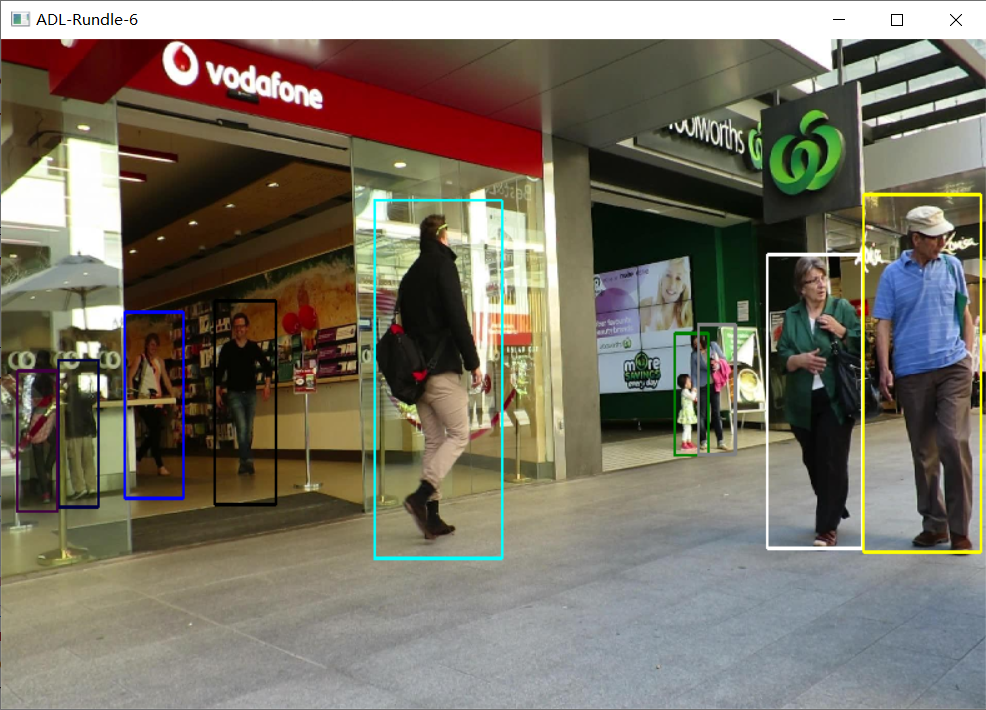
\includegraphics[width=0.8\textwidth]{images/sort.png}
\end{figure}


2. RoboMaster比赛准备

顺利将RoboMaster比赛的模拟器部署,测试了提供的基本服务起飞降落,运行了Faster-LIO实现激光雷达的定位。

\begin{figure}[h!]
	\centering
	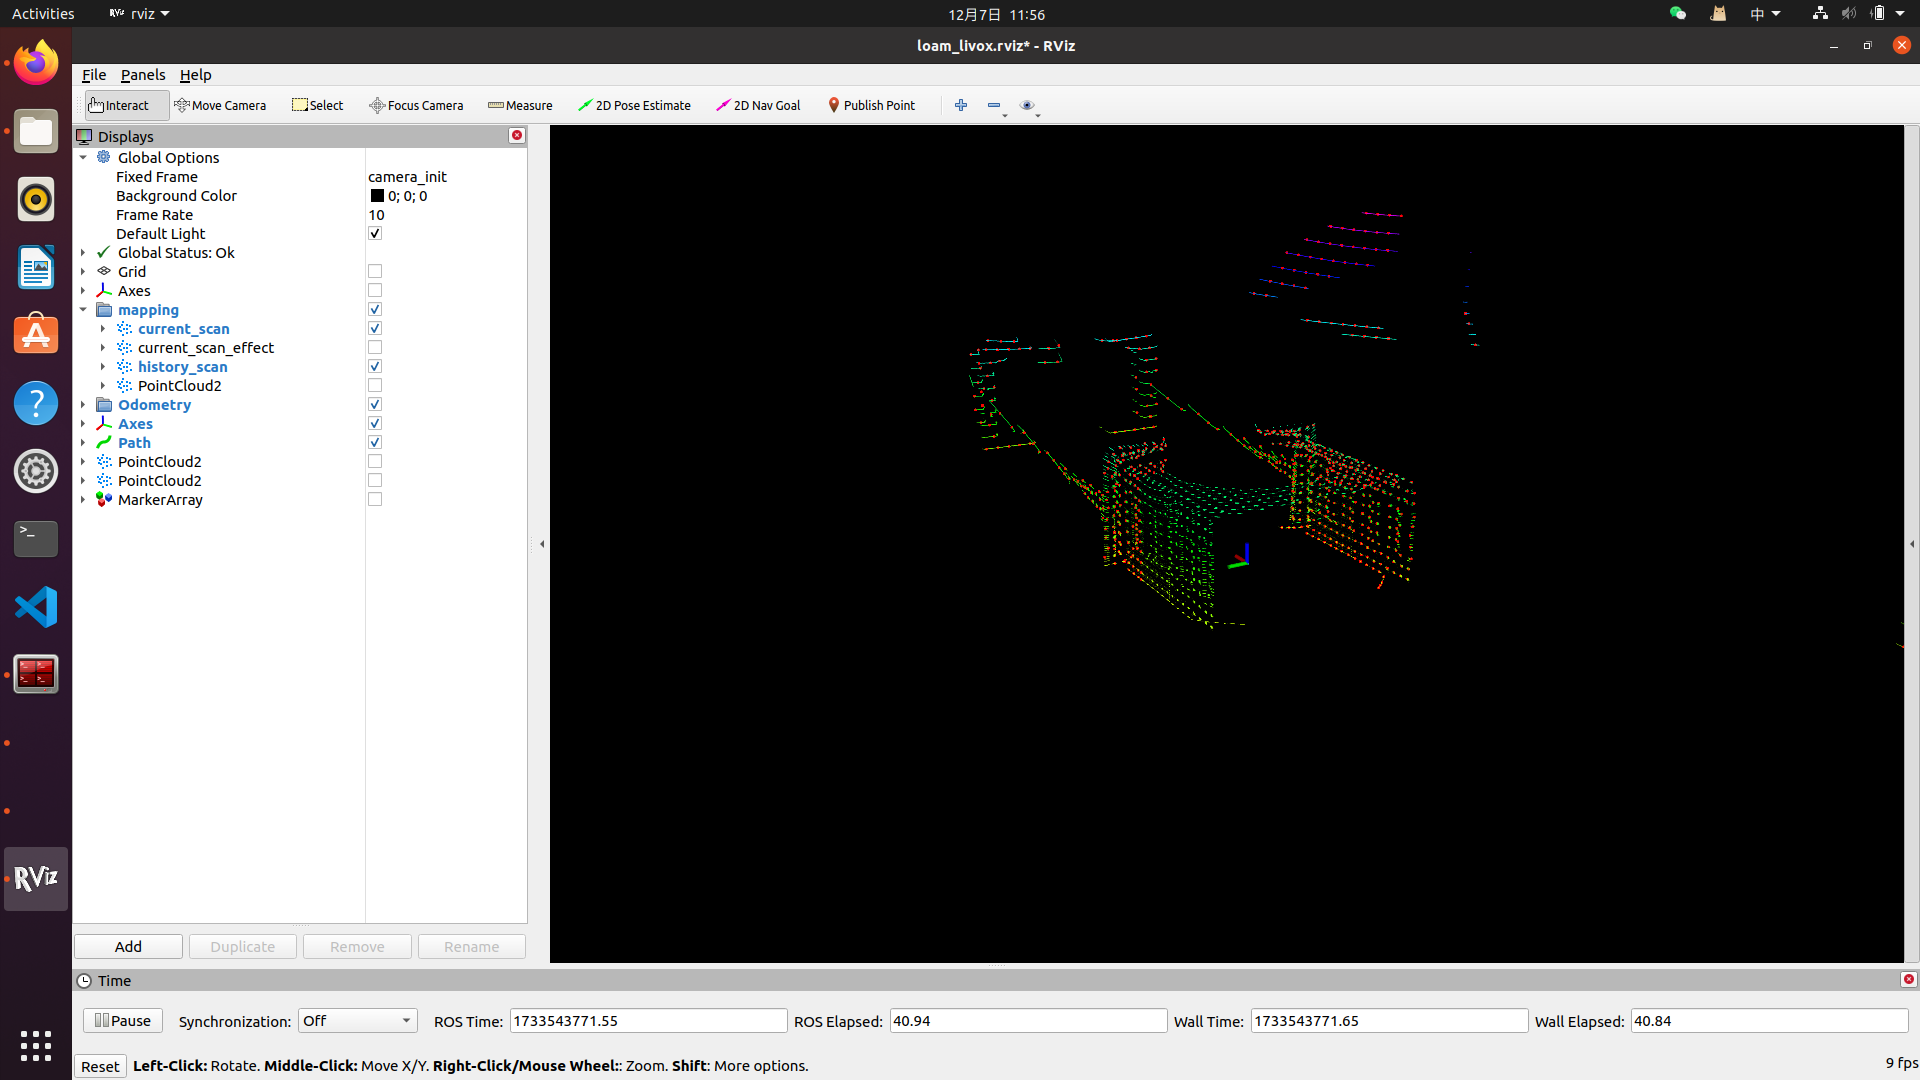
\includegraphics[width=0.8\textwidth]{images/robo/lio.png}
\end{figure}


\chapter{测量指标}
1. 匹配单个结果

正负例(positive/negative)的是依据预测值,真假(True/False)是依据实际值。

\begin{table}[h!]
	\centering
	\caption{基本概念}
	\label{tab:confusion_matrix}
	\begin{tabular}{l c c}
		\toprule
		& \textbf{预测正例} & \textbf{预测负例} \\
		\midrule
		\textbf{实际正例} & TP & FN \\
		\textbf{实际负例} & FP & TN \\
		\bottomrule
	\end{tabular}
\end{table}

2. 召回率

召回率(Recall)是指在所有实际正例中,被模型正确预测为正例的比例。其数学表达式如下:

\[
\text{Recall} = \frac{\text{TP}}{\text{TP} + \text{FN}}
\]




